\chapter{Results and Discussion}
\label{chap:five}
In this section we will discuss the results obtained from 
the performed experiments. We particularly discuss the 
overfitting phenomenon, which is a common problem
for small sample sizes and for low signal to noise problems. 
In the discussion we will compare our
results with similar studies
and further comment on the 
contribution of our study.

\section{Results Intepretation}
\label{sec:results}
In order to assess potential variable importance
we have evaluated a correlation matrix for the initial
dataset, please see Figure \ref{fig:Corr_btc}. High 
levels of multicollinearity highlight the importance of
regularization techniques to avoid overfitting.

\begin{figure}[!h]
    \centering
    \caption{Correlation matrix of the BTC dataset shows high level of 
    multicollinearity.}
    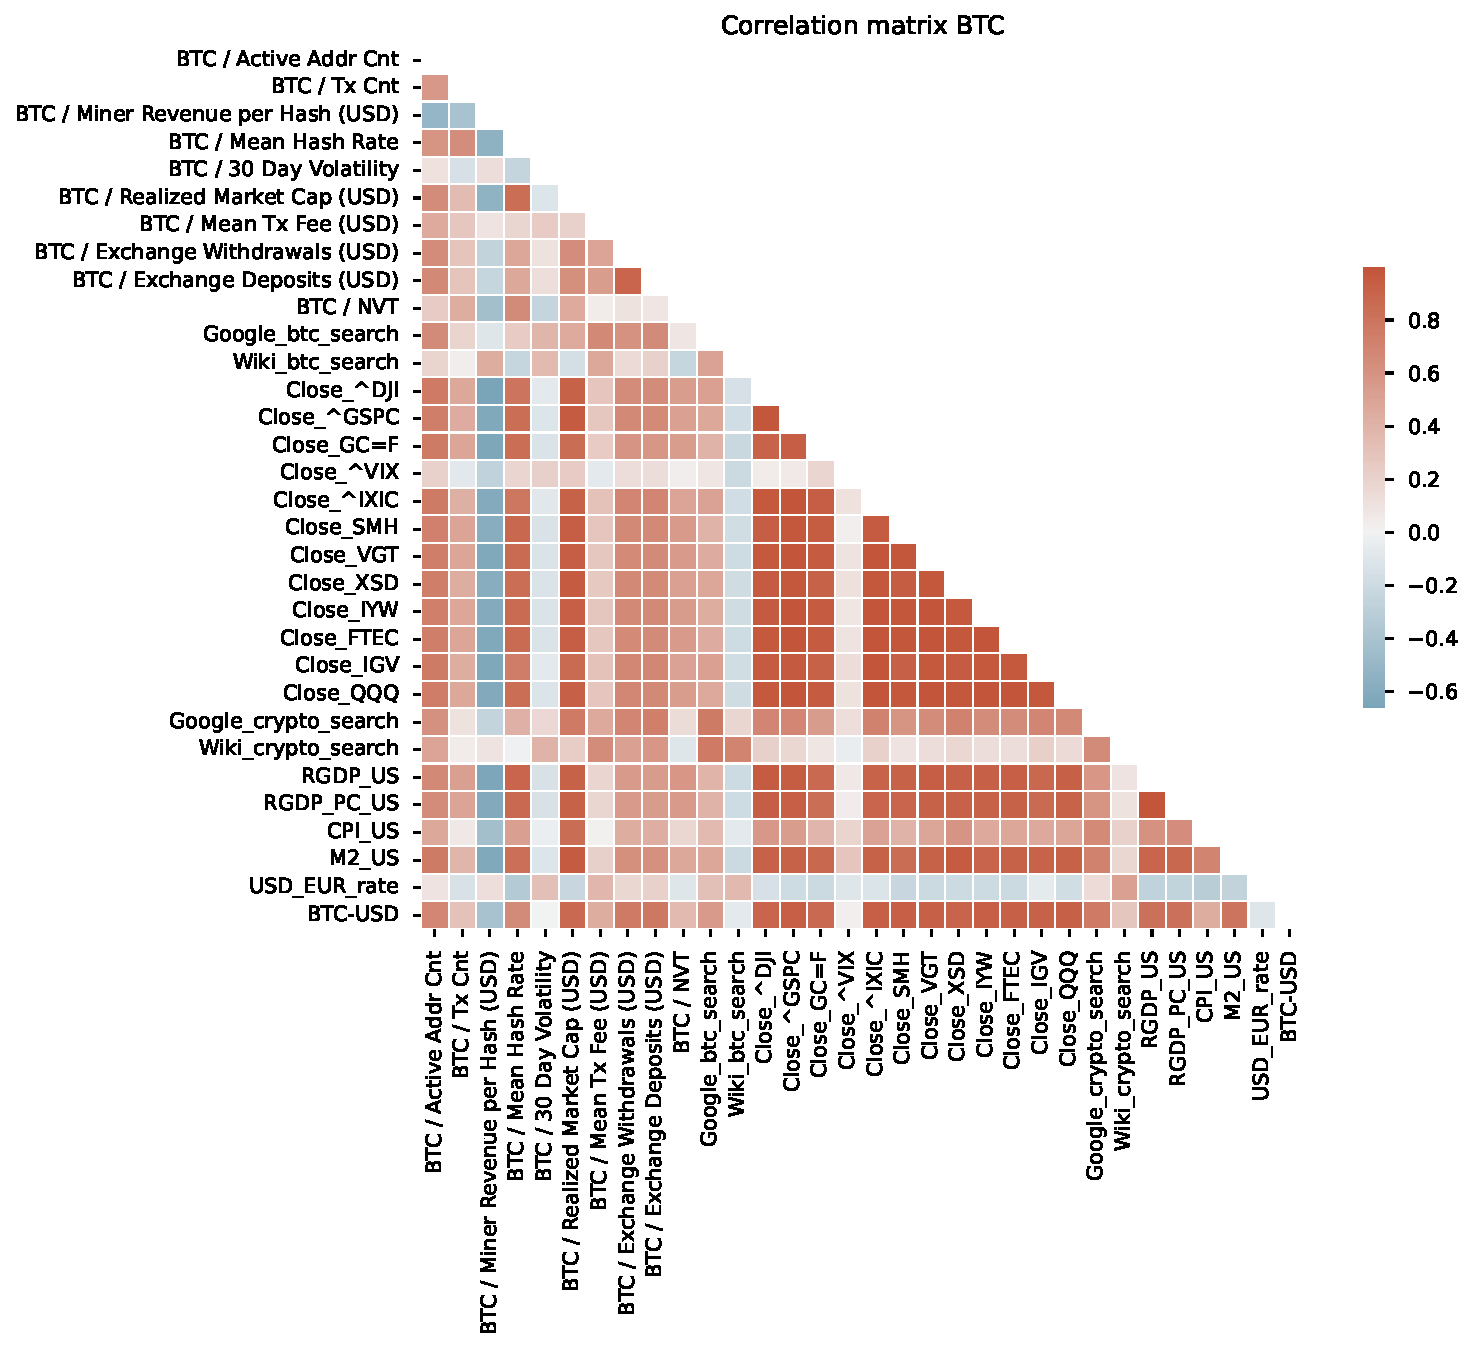
\includegraphics[width=1\textwidth]{Figures/Corr_btc.pdf}
    \caption*{Source: Author}
    \label{fig:Corr_btc}
\end{figure}

Initially, we intended to focus mainly on the price forecasting problem.
After running many experiments with unsatisfactory results, we decided to add 
a set of technical indicators calculated from the price variable.
Concretely, we added the following indicators: simple moving average (SMA) \ref{eq:sma},
exponential moving average (EMA) \ref{eq:ema}, relative strength index (RSI) \ref{eq:rsi} and 
bollinger bands (BB) \ref{eq:bbands}. 
The reason for this decision being the presence
of strong autocorrelation in the target variable which
might be a signal of limited impact of the fundamental pricing side. 




\begin{equation}\label{eq:sma}
    \text{SMA}_t = \frac{1}{w} \sum_{i=0}^{w-1} P_{t-i}
\end{equation}

\begin{equation}\label{eq:ema}
    \text{EMA}_t = \alpha P_t + (1 - \alpha) \text{EMA}_{t-1}, \quad \text{where} \quad \alpha = \frac{2}{w + 1}
\end{equation}

\begin{equation}\label{eq:rsi_avg}
    \text{AvgGain}_t = \frac{1}{w} \sum_{i=1}^{w} \max(\Delta P_{t-i}, 0), \quad
    \text{AvgLoss}_t = \frac{1}{w} \sum_{i=1}^{w} \max(-\Delta P_{t-i}, 0)
\end{equation}

\begin{equation}\label{eq:rsi}
    \text{RS}_t = \frac{\text{AvgGain}_t}{\text{AvgLoss}_t}, \quad
    \text{RSI}_t = 100 - \left( \frac{100}{1 + \text{RS}_t} \right)
\end{equation}

\begin{equation}\label{eq:bbands}
    \text{Upper}_t = \text{SMA}_t + k \cdot \sigma_t, \quad
    \text{Lower}_t = \text{SMA}_t - k \cdot \sigma_t
\end{equation}

After adding the technical indicators, the results
did not improve significantly and the model 
was always converging to the prediction of the current price
which leads to a typical pattern in the 
graph when putting the predicted and actual prices into comparison 
where the prediction is essentially
the target price shifted by the prediction horizon.
Interestinly, this behaviour was observed
even in the case where the model does not know
the current price. However, it was able
to infer it most likely from the capitalization variable or some
other highly correlated variable.
We test this hypothesis by comparing
the model with the naive forecast which predicts the last
observed price and charaterizes
the random walk model. The naive forecast outperforms 
the model in most of the cases on the test dataset. 


In the following steps we decided to focus on the prediction
of log returns. The log returns are calculated as follows:
\begin{equation}\label{eq:log_returns}
    r_t = \log(P_{t+h}) - \log(P_t) = \log\left(\frac{P_{t+h}}{P_t}\right)
\end{equation}

where $P_t$ is the price at time $t$ and $h$ is the time horizon.
The idea behind this approach is that the log returns are stationary in nature
and the model can thus better capture
the pricing dynamics without learning the long term trend.
Thanks to log returns stationarity, 
$R^2$ is a reasonable measure of the model performance that
tells whether the model is better than the naive mean forecast.
Positive $R^2$ indicates that the model is better than the mean forecast.
From a different view, $R^2$ is a relatively strict measure
when the returns shift systematically in one direction on the test dataset.
The reason is that the sum of squares total
is calculated on the test data and thus knowing the test data mean.
However, the models trained on the training dataset do not 
capture this shift as they do not know the test data mean.
Despite that we believe that $R^2$ is a reasonable measure
as the models should be able to outperform this baseline.
Unfortunately, this problem reformulation 
did not help much and the model was still
unable to generalize well to the test dataset despite
decent performance on the training dataset.
It is worth noting that most of our
models have lower root mean square error on the test
dataset than on the training dataset so they 
are not truly overfitting the training data in a typical manner.



We suggest multiple reasons for this behavior. 
Either the signal to noise ratio is too low
and the model is not able 
to learn the pricing dynamics. 
The second reason is that the model is overfitting the training
data despite extremely strong regularization of many forms and
cross validation. We suspect
that the combination of the small sample size and the
nature of the cross validation 
are the main reasons for this behaviour. 

For time series data, the temporal ordering of the data is important.
That is the reason why one should not use the standard cross validation
in order to avoid data leakage especially 
for the scalers that scale the data into a range
which is required by some models. In practice, 
one can use normal cross validation on the training dataset
but it will most likely lead to overfitting.
The second option is to use the time series cross validation
which incrementally increases the training dataset 
and evaluates the model on the next batch of the data.
This approach is more robust but has its own limitations.
The first one is that when the sample size is small, 
the performance of the model is very noisy across the folds
which makes it difficult to evaluate the best hyperparameters. 
Furthermore, varying sample size actually 
lead to different number of gradient descent iterations
for some models which affects the choice of the best hyperparameters.
The second weakness is paradoxically what
makes this approach robust and that is the
act of masking the future distribution of the data.
As most machine learning models and certainly 
those used in our experiments including the \ac{PCA} step
expect the data to be standardized
or scaled to some predefined range.
When the distribution of the data changes
significantly, the scalers trained on the training dataset
will cause the test data to be scaled
outside of those expected ranges and thus breaking the 
performance of the model. 
Unfortunately,
this is the nature of our data 
and shows some limitations of the machine learning approach 
for problems that are changing dramatically over time.


Due to afforementioned problems, we opted for a different approach
which includes differencing and applying logarithm to all of
the independent variables to push them closer to stationarity.
This obviously leads to loss of information 
but may help with the cross validation problem.
Especially, variables that come in weekly and monthly frequencies
and are thus interpolated to daily frequency
will be zero most of the time and thus
may introduce a lot of variance on the edges where the values
are changing. For the correlation matrix of this transformed 
dataset see Figure \ref{fig:Corr_btc_logdiff}. We can 
observe that the correlation levels between the independent variables
and the target variable are really low with highest 
levels being with the technical indicators.

\begin{figure}[!h]
    \centering
    \caption{Correlation matrix of the BTC dataset after
    log differencing all of the variables.}
    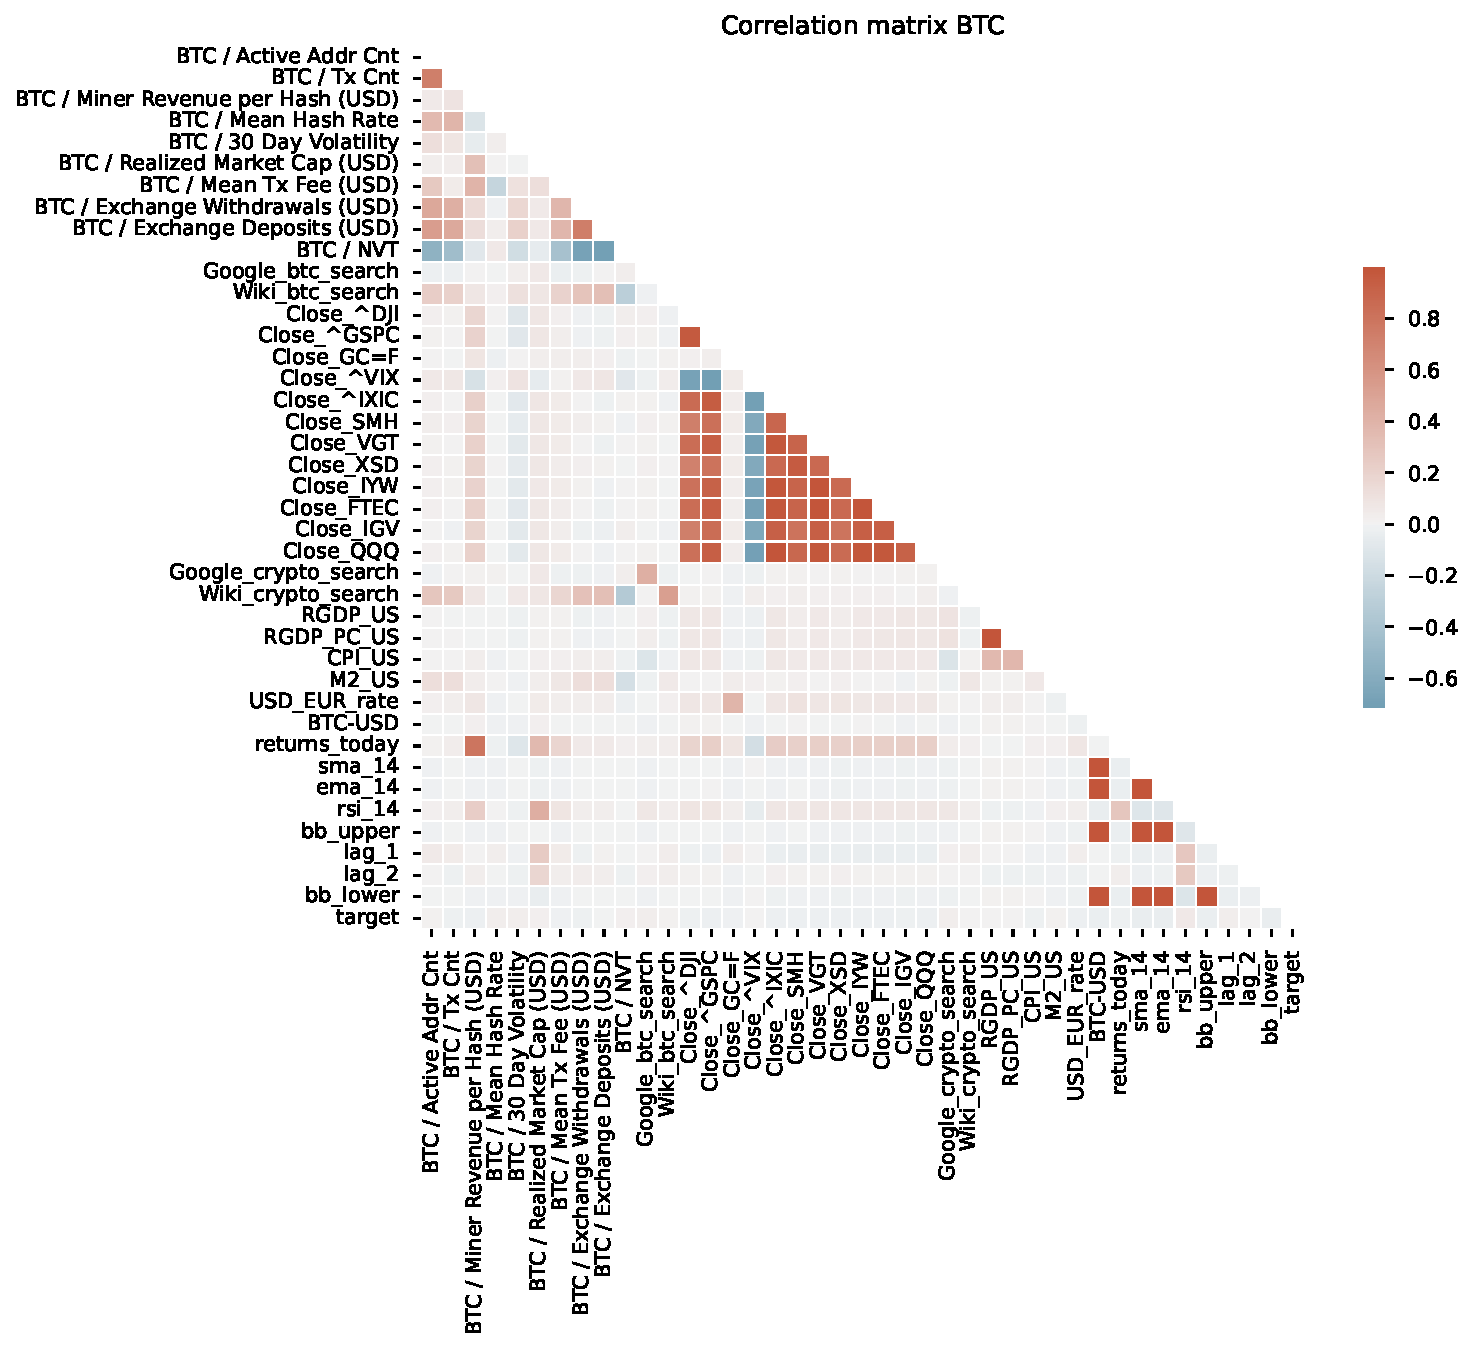
\includegraphics[width=1\textwidth]{Figures/Corr_btc_logdiff.pdf}
    \caption*{Source: Author}
    \label{fig:Corr_btc_logdiff}
\end{figure}

After changing the model specification, we repeated the experiments
using Bayesian cross validation which is 
an advanced technique that 
usually converges faster to better hyperparameters than the standard
grid search cross validation that samples hyperparameters unconditionally. 
We studied the effect of hyperparamters on the model performance
and found that the results are mostly insensitive to the choice of the
hyperparameters except the \ac{LSTM} network. As a result, cross validation tends to 
select highly regularized models that 
are not able to learn the training data well and only predict the mean value.
This is a typical sign of overfitting to the training noise and
not to the signal. 


As cryptomarket is characterized by significant structural breaks
that shift the distribution of the data, we wanted
to test whether the model is able to generalize well
until the highly volatile period of 2021. We decided to cut 
the dataset at the beginning of 2021 and rerun the experiments.
To our suprise, the results were not significantly different and the 
generalization performance was still very poor.


We suspect that the signal to noise ratio is too low
or the the pricing dynamics are changing too often 
which leads to the inability of the model to generalize
to out-of-sample time periods. We inspect the latter hypothesis
on the example of the learned coefficients of the Ridge regression model
with incremental training that represents
the time series split and the sliding window approach that represents
the true changes in the dynamics in time.
The learned coefficients are shown 
in Figures \ref{fig:coefs_incremental_btc} and \ref{fig:coefs_sliding_btc},
where the coefficients with highest variance are highlighted.
We can observe that the coefficients are changing over time relatively
dramatically which explains the poor performance of the model. Obviously,
some variance is expected due to the low size of these folds
that causes noisiness in the learned coefficients especially in the sliding
window approach. Similar results were obtained for the other cryptocurrencies.
To see the final results tables see Appendix \ref{app:A}.


\begin{figure}[!h]
    \centering
    \caption{Learned coefficients of the Ridge regression model
    with incremental training on the BTC dataset. Five 
    coefficients with highest variance are highlighted.}
    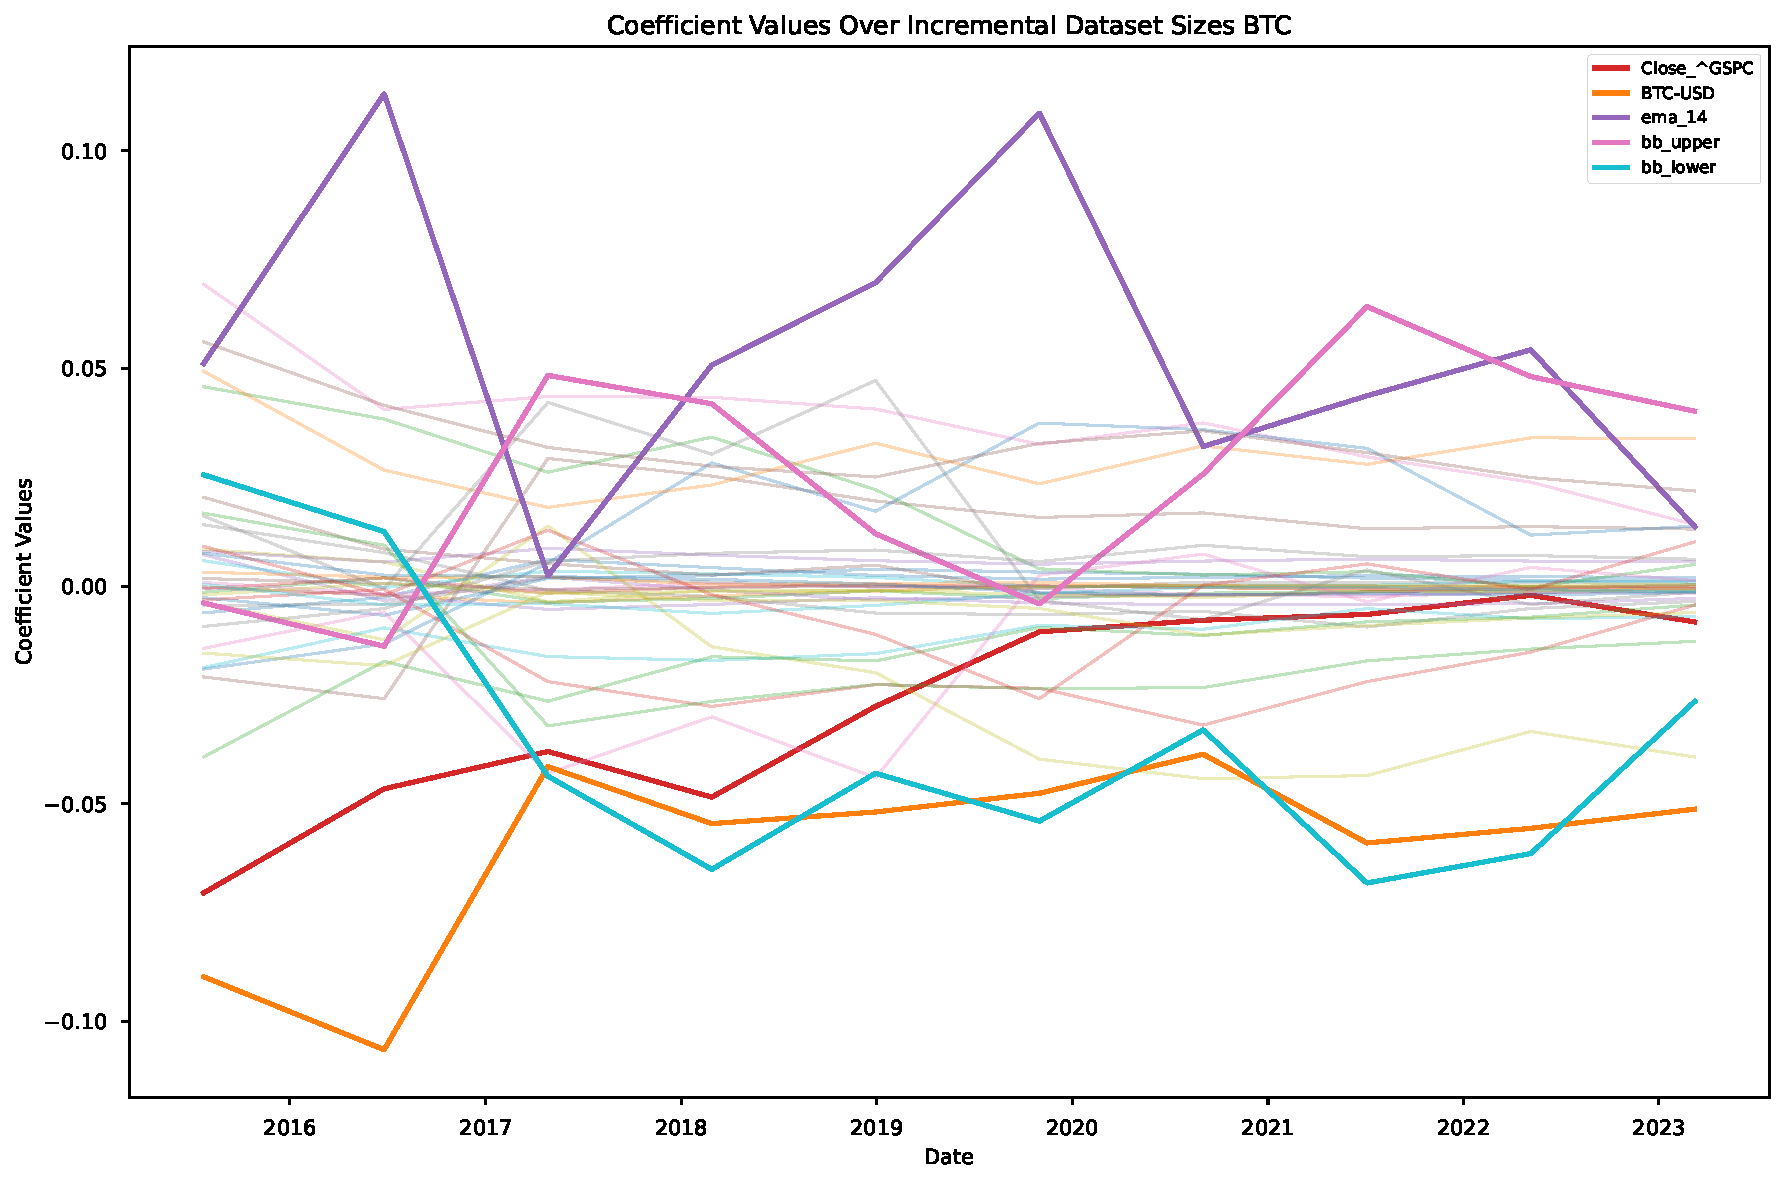
\includegraphics[width=1\textwidth]{Figures/coefficient_values_incremental_btc.pdf}
    \caption*{Source: Author}
    \label{fig:coefs_incremental_btc}
\end{figure}

\begin{figure}[!h]
    \centering
    \caption{Learned coefficients of the Ridge regression model
    with sliding window training on the BTC dataset. Five 
    coefficients with highest variance are highlighted.}
    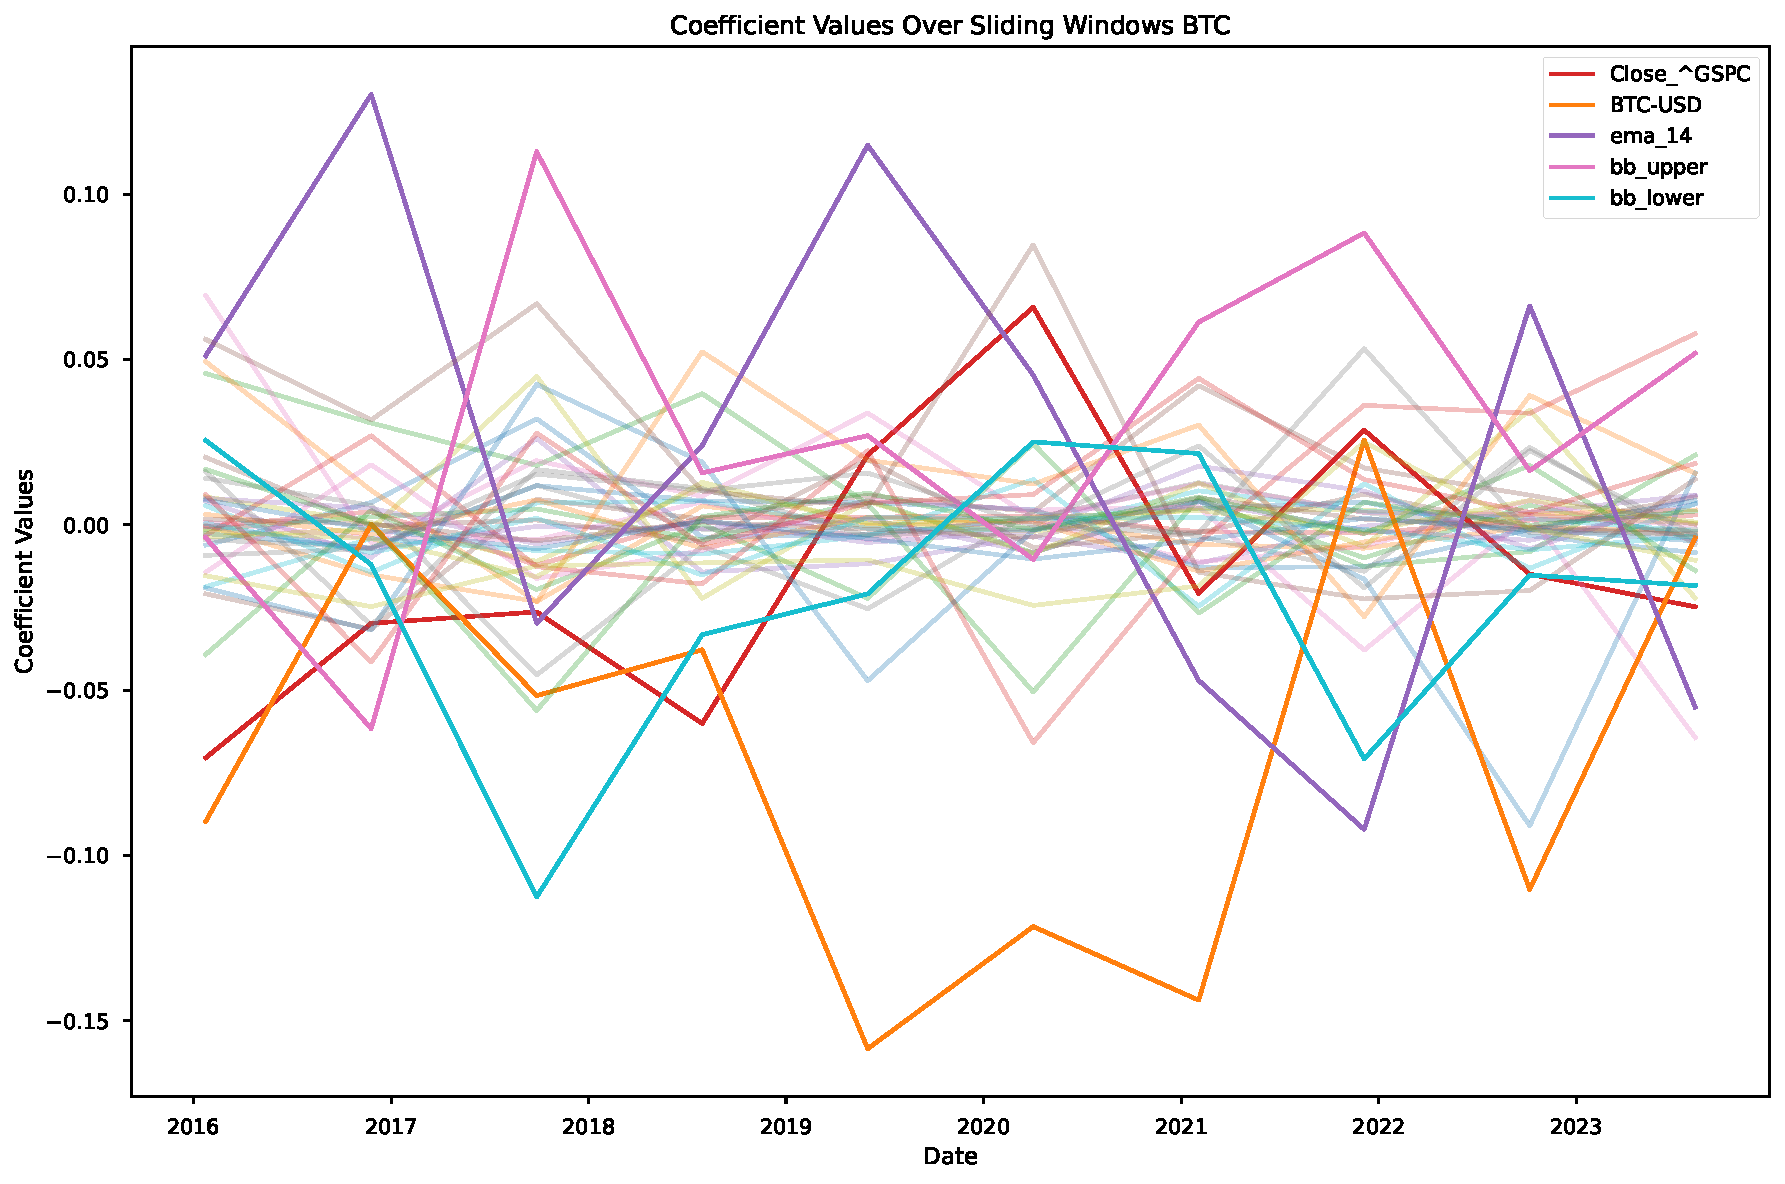
\includegraphics[width=1\textwidth]{Figures/coefficient_values_sliding_btc.pdf}
    \caption*{Source: Author}
    \label{fig:coefs_sliding_btc}
\end{figure}

\section{Limitations}
\label{sec:limitations}
Unfortunately, the poor model performance 
prevents us from making any conclusions about the
initial hypothesis of the thesis. The results 
are not significantly different even with the \ac{PCA}
layer added. However, there seems
to be some limited evidence for less overfitting behaviour 
in the case of the \ac{PCA} model
but the results are still worse than the naive forecast leading to
negative $R^2$ on the test dataset. We conclude
that the model is not able to learn the pricing dynamics
due to the low signal to noise ratio and the changing pricing dynamics.


Our study is limited by the choice and 
quality of the data. Despite having 
a lot of variables representing the network activity and 
other fundamental variables, the quality of the trend data is low.
Only the wikipedia page views come in daily frequency
but we did not expect this variable to be especially informative. 
Whereas Google trends data were available in weekly frequency
which leads to low information for daily forecasting.
We believe that better data quality would improve
the model performance significantly. 
Secondly, there might exist a better combination of technical
indicators that would help the model to learn the pricing dynamics.
Finally, more advanced techniques to increase
the dataset size such as generative adversarial networks 
might help to improve the generalizability properties of the model.

\section{Discussion}
\label{sec:discussion}

In this section we provide a brief discussion
of the results with respect to the existing literature.
As we have already mentioned, we have previously
identified many problematic treatments of 
similar topics in the literature. We believe
that our study is taking a broader 
perspective aggregating knowledge
from multiple previous experiments especially from the data perspective. 
Our contribution is primarily on the 
methodological side where we focus 
in detail on the data preprocessing steps and 
on multiple phenomena regarding specifics
of non-stationary time series that are often neglected in the literature.
It is thus relatively difficult to compare our results with
the existing literature as 
some of the studies are using different data
or do not publish the code used for the experiments.

Similar study to ours by 
\cite{Liu2023} suggests
that they were able to obtain out-of-sample $R^2$  of 4.8\%
which is significantly better than our results.
But there are some important findings from their study
that actually correlate with our findings.
Firstly, their results were extremely 
dependent on the choice of model where the XGBoost model
with only one feature being 1-day lagged returns outperformed 
other models. 
Secondly, they run the experiment
for 3703 different cryptocurrencies and find out 
that there is some predictability in the small
cryptocurrencies but not in the large ones. This
is in line with our findings where
we do not study different cryptocurrencies due to data limitations.


A different study by
\cite{Yae2022} focused on the properties
of different algorithms for out-of-sample returns forecasting
for Bitcoin, Ripple and Ethereum. 
They find out that only the change in stochastic correlation with the stock
market is able to predict the returns with statistical significance.
Whereas other models including \ac{ML} models 
are not able to outperform the naive forecast. 
They highlight the importance of out-of-sample testing
as most of the analyses in the literature are based on in-sample evaluations.
This opens up the door for future research focusing
on the out-of-sample performance of traditional econometric and other models
which are usually fitted on the entire dataset and their generalizability 
might be limited. This study 
uses a better evaluation metric than traditional $R^2$ 
which is $R^2$ against historical averages and $R^2$ against zeros
which might be a more forgiving measure of the model performance.
Despite that, 
most of the \ac{ML} model they have studied score negative $R^2$ on 
the test dataset.

An older study by \cite{Akyildirim2020} 
used a different approach 
where they used many \ac{ML} models to predict
whether the returns will be positive or negative. 
They find out that the \ac{ML} models are able to outperform 
the 50\% accuracy baseline however 
it is not entirely clear how the test dataset was constructed with
respect to the time dimension. Furthermore, 
the choice of the baseline should be validated
by some analysis of the proportion of positive and negative returns.
Unfortunately, the literature on
this topic is relatively scarce. This might mean
that either the topic is not very popular or that the results are not worth
publishing. It is however to draw any conclusion which is the case.

We still believe that there is some potential in the \ac{ML} models
but there is a need for better data quality and for models
that directly model the economics aspects of the problem
as the basic data science workflow does not seem 
to be sufficient for this problem.




